
%%%%%%%%%%
\section{System Overview}

In order to provide control of our small optic suspensions, we had the option of building either a digital or analog feedback system.
Although either option would work for the experiment the digital system provides additional benifits:

\begin{enumerate}
\item Easy modification of feedback loops
\item Builds Familiarity to LIGO digital systems
\item Can be used as a platform for testing new LIGO tools
\item A platform for rapid implementation of future control loops
\end{enumerate}

The digital system employed at Syracuse closely resembles the LIGO digital system. It is composed of the following major components:
\begin{enumerate}
\item Real-time Front-end for digital feedback and control
\item ADC and DAC for interfacing digital system with the experiment
\item Data Acquisition
\item Workstation for controlling the experiment, running tests, and analyzing data
\item Boot server for serving the diskless front-end machine
\end{enumerate}

\begin{figure}[htbp]
	\centering
		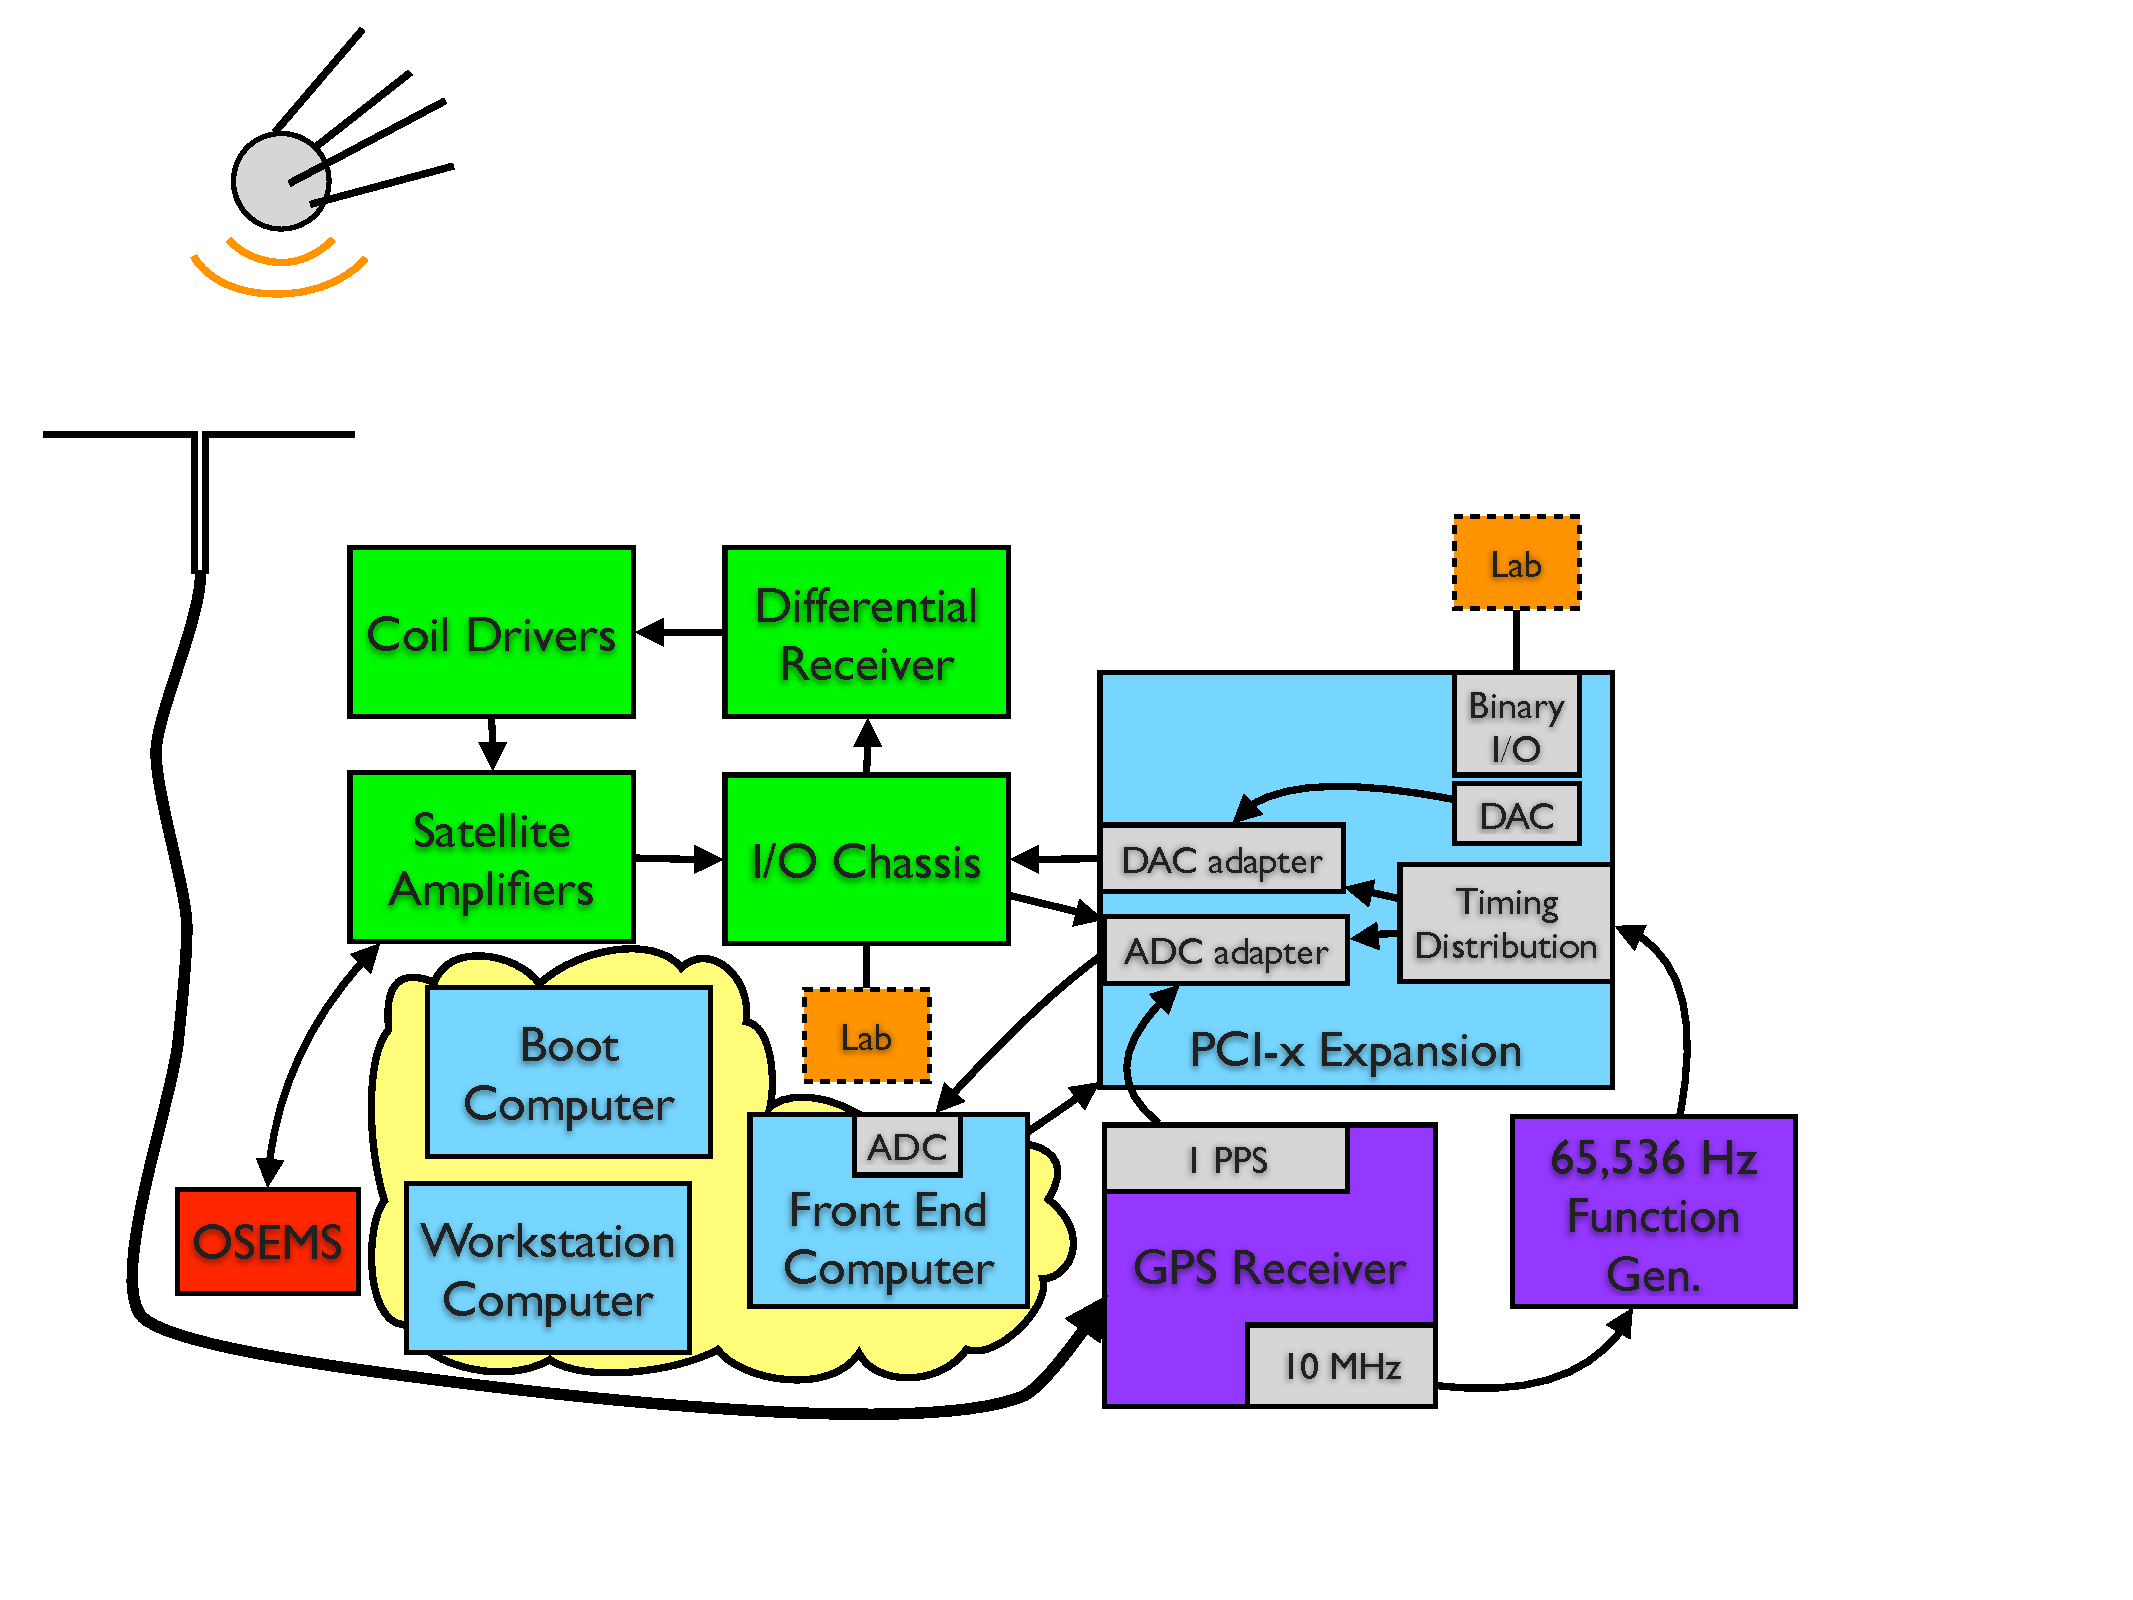
\includegraphics[width=15cm]{./figures/FrontEndSystem.pdf}
	\caption[Front End System Overview]{Front End System Overview}
	\label{fig:front_end}
\end{figure}

\begin{table}
\begin{center}
\begin{tabular}{ | l | l | l | }
\hline
From & To & Connection \\
\hline
Front-End Computer & ADC card & PCIe bus \\
Front-End Computer & Expansion Chassis & PCIe to PCIx adapter \\
Expansion Chassis & DAC card & PCIx bus \\
ADC card & ADC adapter card & SCSI cable \\
DAC card & DAC adapter card & SCSI cable \\
Expansion Chassis & Binary I/O cards & PCIx bus \\
Timing Distribution Card & ADC card & coaxial SMB \\
Timing Distribution Card & DAC card & coaxial SMB \\
Function Generator & Timing Distribution Card & BNC \\
GPS Receiver & Function Generator & 10 MHz sync BNC \\
GPS Receiver & ADC adapter card & 1PPS BNC \\
\hline
\end{tabular}
\end{center}
\caption[Digital System Hardware Interface Matrix]{This interface matrix depicts
the physical interconnectivity of digital system hardware components.
}
\end{table}

%%%%%
\subsection{LIGO Real-Time System Theory of Operation}

The LIGO Real-Time System provides for discrete, synchronous control of LIGO
systems. The sampling frequency can be one of several powers of 2 in Hz.
Time is synchronized to GPS time with a sophisticated timing distribution
system. The digital processes are run in fixed time steps in order to run
feedback signals through them which are analogous to continuous time feedback
systems. One can then design a feedback system composed of poles and zeros
completely inside the computer. The limitation being that of a bandwidth below
the Nyquist frequency for the sampling rate used.

Timing signals are received by the digital system through the ADC/DAC cards.
Each model has a limited time to process the data before the next time step
begins.


%%%%%
\subsection{ADC/DAC Hardware Description}

%%%%%
\subsection{Timing}

Time steps must be spaced precisely enough to avoid jitter (a phase noise
associated with a variable time step). In practice it is impossible to
avoid, but we can minimize jitter by referencing a crystal oscillator.
Crystal oscillators are notoriously precise by using the natural mechanical 
oscillations of crystals which have very low mechanical loss.

The timing signal for the front end system is directly generated by a Stanford Research DS345 function generator. It produces a 65,536 Hz signal that clocks the ADC and DAC cards. Over a long period of time the time stamp in the front end can drift relative to the computers that are synced to network time. Some software, particularly Diagnostic Test Tools and probably others, gets confused when the current time in front end does not match network time. This requires a reboot of the front end system to reacquire the correct time.

We ordered a GPS receiver (Trimble Thunderbolt E) that will prevent these long term drifts. It produces a 1PPS (Pulse Per Second) signal and a 10 MHz signal. The 1PPS connects to the ADC card through the ADC adapter card which is located in the blue expansion chassis. The 10 MHz signal connects to the external timebase input of the DS345. So, the 65,536 clock is now "disciplined" to the GPS time and as such should not drift over long periods of time.

Additionally, the Thunderbolt has an ovenized crystal oscillator that should help with phase noise.

In order to get the GPS antenna signal we needed about 250' of low-loss 1/2" diameter foam core cable (should be easy to spot as it's quite thick). The cable runs out the optics lab, across the hallway overhead and into a cable tray to go down the hallway. The cable runs out of the cable tray by the machine shop, over the hallway, into the machine shop, up to the ceiling, and then along the top of a black drain pipe to the south-east corner of the building. The cable then goes through some grating on the wall and up the shaft to the ground level of the SE corner where the antenna is mounted. (see Fig.\ref{fig:gps_antenna})

\begin{figure}[htbp]
	\centering
		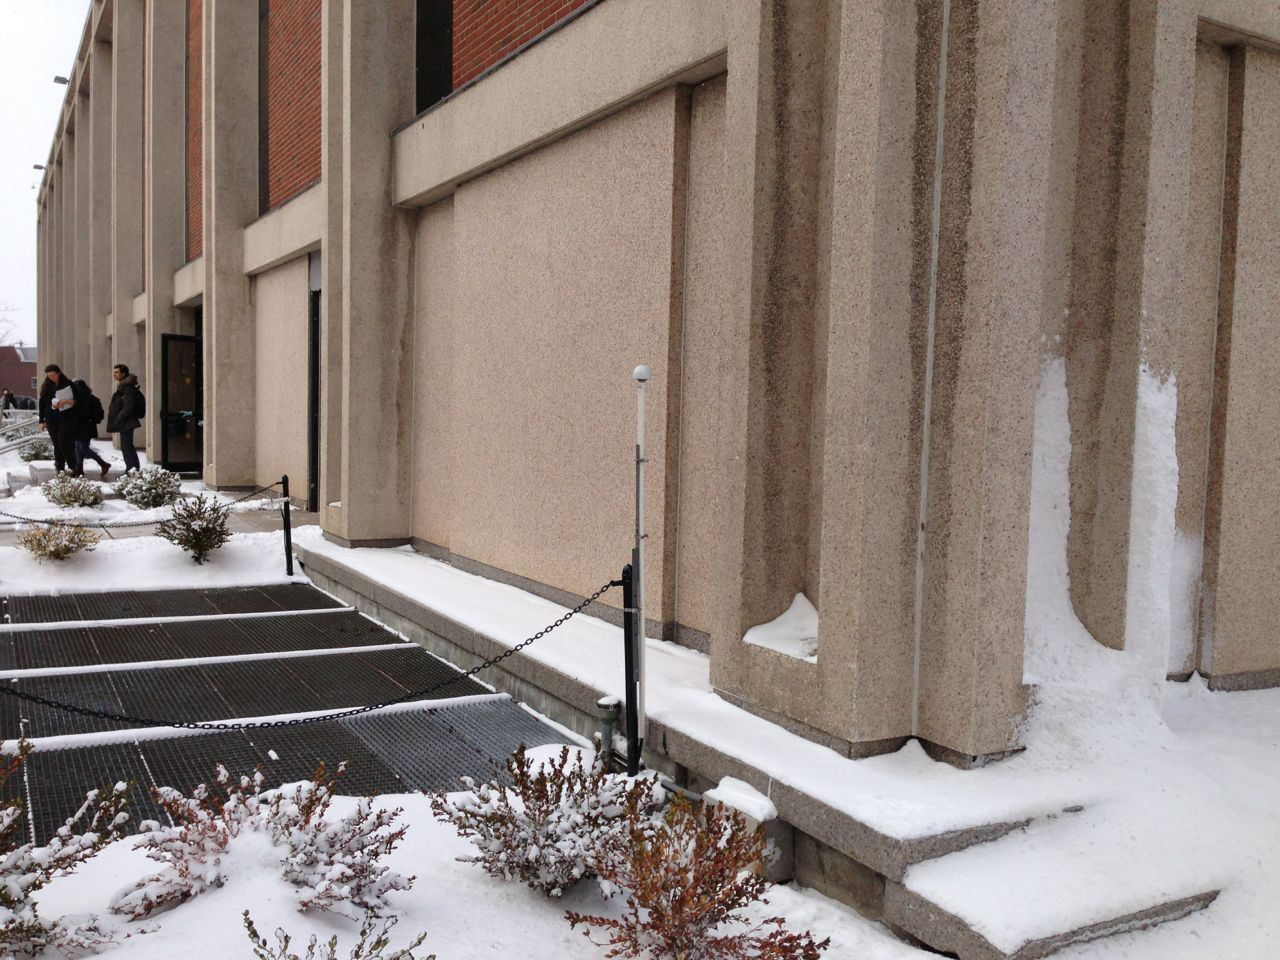
\includegraphics[width=15cm]{./figures/IMG_1308.jpg}
	\caption[GPS Antenna Location]{The GPS antenna is located }
	\label{fig:gps_antenna}
\end{figure}

The 1PPS signal from the Trimble Thunderbolt GPS receiver is a fixed pulse width of 10 micro-seconds. Since the clock is running at 65,536 Hz, the 1PPS is missed by the ADC.

I have fixed this by extending the pulse to about 15 microseconds using a 555 timer chip in monostable mode. The input has to be an inverse pulse so I inverted the pulse in GPS control software. This option is available in the Timing Receiver Configuration window.

See attached NE555P spec sheet (p.9) for the schematic that I used. Only difference is $R_L$ is between output and ground instead of $V_{CC}$.

I scavenged a 5V power supply from an old 10baseT ethernet hub. I took the ferrites and electrolytic capacitor that were on the supply input in the hub itself and added them to this board for noise suppression.

$R_A$ is a small potentiometer. If you need to adjust the pulse width, just open the case and turn the pot. Clockwise increases the width.

\begin{figure}[htbp]
	\centering
		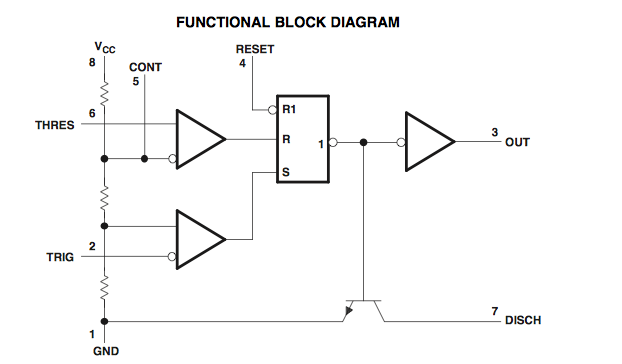
\includegraphics[width=15cm]{./figures/timer555.png}
	\caption[555 Timer Diagram]{This block diagram depicts the function of the 555 timer. The }
	\label{fig:timer_diag}
\end{figure}


\begin{figure}[htbp]
	\centering
		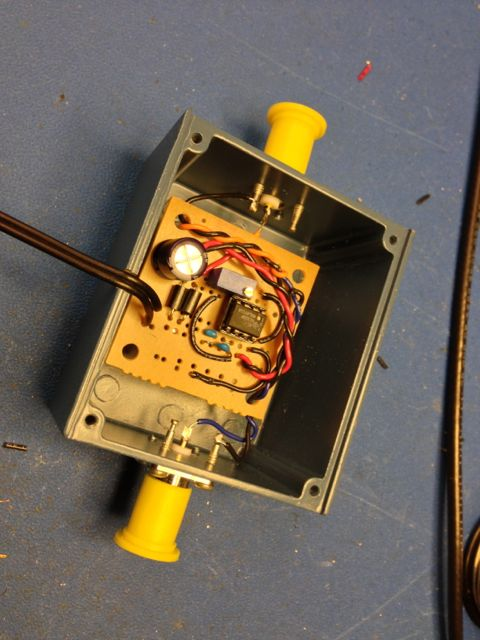
\includegraphics[width=15cm]{./figures/IMG_1345.jpg}
	\caption{{GPS Pulse Extender}}
	\label{fig:gps_pulse}
\end{figure}

The first thing to check in the GPS software is the status. It should say "over-determined clock". Other key items in the control software to pay attention to are basically the number of green lights (in this case 5) and the holdover time in the upper-right window labeled "Timing Receiver Status and Control". If things are working correctly the number of green satellites will typically be 4-5 with the antenna at it's current location. We should also not see any holdover time. When the receiver is not using any satellites it enters a "holdover" state where the oscillator is no longer disciplining. The GPS keeps track of how long it's been in holdover. Going into holdover could indicate a problem in the connection to the GPS antenna.


%%%%%%%%%%
\section{Front-End Code Installation}

We have acquired a clone of the front end disk used at Livingston. The disk was backed up locally (sugar-dev3:/lab/frontend/sata-disk-backups/mnt2 as of 2013/02/18). The disk was adapted for use at Syracuse. The disk failed on 6 Feb 2013. This page documents the second build of the front end at syracuse...



%%%%%
\subsection{Using LLO Cloned Disk}

The cloned disk is saved in \lstin?/lab/frontend/sata-disk-backups/mnt2? and a tar file
of the contents was made on
\todo{insert date}. We use the tar file from LLO to build a new machine. The new machine
can either be used to serve a diskless front-end machine or used as a standalone front-end
machine.


\subsubsection{Diskless Node Install}

\begin{enumerate}
    \item Acquire machine with same architecture as front-end (presumably x86\_64).
    \item Login using gentoo minimal-CD or Live-DVD.
    \item Repartition first disk (/dev/sda) to one partition and create ext3 filesystem.
    \item Make mount point for sda1 and mount.
%
\begin{lstlisting}
mkdir /mnt/fe
mount /dev/sda1 /mnt/fe
\end{lstlisting}
%
    \item Make mount point for /lab and mount directory.

\begin{lstlisting}
mkdir /mnt/lab
mount -t nfs 10.20.1.15:/sugwg/projects/lab /mnt/lab
\end{lstlisting}

    \item copy tar file:

\begin{lstlisting}
rsync -a /mnt/lab/frontend/sata-disk-backups/mnt2/fe.tar.gz /mnt/fe/
\end{lstlisting}

    \item untar file:

\begin{lstlisting}
cd /mnt
tar -xvf fe/fe.tar.gz
\end{lstlisting}

    \item chroot into new filesystem and setup for use on network...

\begin{lstlisting}
mount -t proc proc /mnt/fe/proc
mount --rbind /sys /mnt/fe/sys
mount --rbind /dev /mnt/fe/dev
chroot /mtn/fe /bin/bash
source /etc/profile
\end{lstlisting}
\end{enumerate}
\todo[inline,color=red]{Add networking configuration details}


\subsubsection{Local Disk Install}

%%%%%
\subsection{Minimal tar deploy}

Create a tar file without the portage, front-end target, and cvs/svn directories...

\subsubsection{Creating tar file for Syracuse front-end machine}

This is the procedure used to create an archive of a front-end system modified for use at Syracuse. Here, I am using 10.20.1.44 (s1boot0) as the machine to boot from (the tftp server) and 10.20.1.45 (s1labfe1) is the diskless front-end machine. This can easily be modified for installation directly onto the hard drive.


\begin{enumerate}
    \item Copy the fe tar file to \lstin?${FE_LOCATION}? and untar.
\begin{lstlisting}
cd ${FE_LOCATION}
cp /lab/frontend/sata-disk-backups/mnt2/fe.tar.gz .
tar -xvpf fe.tar.gz
\end{lstlisting}
    \item \lstin?${FE_LOCATION}/fe? is now the root directory for the front-end system
\begin{lstlisting}
export FE_ROOT=${FE_LOCATION}/fe
\end{lstlisting}
    \item At LLO the controls user has UID:GID = 1001:1001. Change this to 512:512 for Syracuse. (You must execute this as root)
\begin{lstlisting}
find ${FE_LOCATION} -xdev -user 1001 -print0 | xargs -0 chown 512:512
\end{lstlisting}
    \item Change the lines for controls in the files \lstin?${FE_ROOT}/etc/passwd? and \lstin?${FE_LOCATION}/fe/etc/group?
    \item Edit \lstin?${FE_ROOT}/etc/ntp.conf?: Change "server" and "restrict" lines and comment out "broadcast" line
\begin{lstlisting}
server 10.20.1.25
restrict 10.20.1.0 mask 255.255.255.0 nomodify nopeer notrap
\end{lstlisting}
    \item Comment out entries in \lstin?${FE_ROOT}/etc/conf.d/net? and add this line:
\begin{lstlisting}
config_eth4=( "10.20.1.45 netmask 255.255.0.0 broadcast 10.20.255.255" )
\end{lstlisting}
    \item Change ip address found in 3 files in \lstin?${FE_ROOT}/etc/xinetd.d/? from \lstin?10.144.0.0/24? to \lstin?10.20.1.0/24?
    \item Comment out 3 lines in \lstin?{FE_ROOT}/etc/resolve.conf?
    \item remove \lstin?${FE_ROOT}/opt/rtcds?
\begin{lstlisting}
rm -rf ${FE_ROOT}/opt/rtcds
\end{lstlisting}
    \item Comment out all lines in fstab except for "shm" and add lines for root and lab.
\begin{lstlisting}[basicstyle=\tiny]
10.20.1.44:/tftpboot/s1labfe1  /    nfs sync,hard,intr,rw,nolock,rsize=8192,wsize=8192 0 0
10.20.1.15:/sugwg/projects/lab /lab nfs sync,hard,intr,rw,nolock,rsize=8192,wsize=8192 0 0
\end{lstlisting}
    \item Change \lstin?EPICS_CA_ADDR_LIST in ${FE_ROOT}/opt/cdscfg? directory
\begin{lstlisting}
find /ligo/feback/fe/opt/cdscfg/ -type f -print0 | xargs -0 sed --in-place=.old s/10.144.0/10.20.255/g
\end{lstlisting}
    \item Comment out \lstin?source /opt/cdscfg/rtsetup.sh? from \lstin?${FE_ROOT}/home/controls/.bashrc? and add the following lines in it's place:
\begin{lstlisting}
export IFO=X2
export ifo=x2
export SITE=TST
export site=tst
export RCG_LIB_PATH=/lab/frontend/controls/git/cds_user_apps/cds/b1/models
export RTCDSROOT=/opt/rtcds/${site}/${ifo}
export NDSSERVER=10.20.1.45:8088
export EPICS_CA_ADDR_LIST="10.20.255.255"
export EPICS_CA_AUTO_ADDR_LIST="NO"
export LD_LIBRARY_PATH=${LD_LIBRARY_PATH}:/lib:/usr/lib:/usr/local/lib:/opt/rtapps/fftw-3.2.2/lib
source /opt/rtapps/epics/etc/epics-user-env.sh
source /opt/rtapps/ldas-tools-1.18.2/etc/ldas-tools-user-env.sh
source /opt/rtapps/libframe-8.11/linux-x86_64/etc/libframe-user-env.sh
source /opt/rtapps/libmetaio-8.2/linux-x86_64/etc/libmetaio-user-env.sh
source /opt/rtapps/gds/etc/gds-user-env.sh
export PATH=${PATH}:/opt/rtapps/dv:/opt/rtcds/${site}/${ifo}/scripts
\end{lstlisting}
\end{enumerate}
\subsubsection{Creating a bootable disk for front-end}

This is how to build a disk that can be installed directly into a front-end machine.

*NOTE* The machine that you build this disk from must have the same type of disk controller as the front-end machine you intend to install this in.

\begin{enumerate}
    \item Locate a spare disk and install in a machine connected to the internal network that you have root access to.
    \item Mount \lstin?/lab? on this machine.
    \item Use fdisk or parted to partition the spare disk.
\begin{lstlisting}
Number  Start   End     Size    Type     File system     Flags
 1      512B    32.0MB  32.0MB  primary  ext2
 2      32.5MB  542MB   510MB   primary  linux-swap(v1)
 3      542MB   1000GB  1000GB  primary  ext4
\end{lstlisting}
    \item Mount \lstin?/dev/sd*? (blank spare disk) at \lstin?/mnt/fe?
\end{enumerate}

\subsection{From Gentoo Source}
Installation from source seems to be ideal, however, there are a few issues
which make it a challenge. At this point this is a theoretical discussion of
how one would do this installation.

The kernel has a special patch to allow the OS to dedicate CPU cores to
front-end models. The earliest supported kernal in the Gentoo source is newer
than the most recent kernel patch for rtcds. The patch involves fewer than 10
lines of code, but it would take some time to figure out how to apply it to
the current version of the kernel and verify it's functionality.

There are numerous library dependencies involved that need to be determined.

%%%%%%%%%%
\section{Front-End Operation}

%%%%%
\subsection{Running a Model}

%%%%%
\subsection{Changing a Filter}

%%%%%
\subsection{Changing a Model}

%%%%%
\subsection{Data Storage}

\subsection{Analysis Tools}


